\section{Active learning (Stage 1)}
\label{sec:visualizer:al}

\subsection{Decision tree classification of user interests}
\label{sec:visualizer:al:tree}

A decision tree is a method of classifying and labeling plots. An ``active learner'' adapts as the process moves forward, choosing its points of query intelligently. Active learning increases efficiency when searching through the hypothesis space, which is any fitted tree that agrees with the labeled data as much as possible~\cite{dasgupta2011}. Every time new data (a new label) is received, the hypothesis space shrinks as the label removes certain classifiers from the running~\cite{dasgupta2011}. An active learner queries from ambiguous parts of the current hypothesis space so as to shrink it as quickly as possible. It is problematic to start from scratch, however; how does the system determine the best first point of ambiguity when it knows nothing (the hypothesis space is everything)? While this problem is difficult, we can exploit the fact that the user is already providing a numerical model that they believe to be a good representation of the data which they would like the visualization system to check visually. Given this data, the system builds a decision tree that utilizes the various properties of the plots to determine whether one is interesting or uninteresting. Doing so greatly narrows the hypothesis space and makes it easier to determine points of ambiguity. However, to reconcile with the fact that the user wishes to check the numerical model and may not necessarily believe it is a good representation of fit, the learner must then perform several line-up tests (Section ~\ref{sec:visualizer:al:lineup}) to check whether the initial decision tree is a proper fit. As the user then proceeds to label various conditional plots as ``interesting'' or ``not interesting,'' the classifier learns the user’s interest and continues to evolve. This models plot characteristics that the user found interesting to study.

\subsection{Rejection classification}
\label{sec:visualizer:al:rejection}

So far, we have been discussing classification as black and white, interesting versus non-interesting. While interacting with the data visually, the user's concept of what's interesting in the specific dataset may evolve over time; at the beginning, they have no idea what the data looks like and where to set the bar for their own standards of dependence. There are several ways to take this into consideration. 

First, the visualization system could assign a weight to the analyst's responses by trial number where the last few plots are more valuable than the first few. However, this may destabilize cases where the user's preferences don’t end up changing, and it is difficult for the classifier to continuously rebalance each round given the weights (which, when applied to 2 black and white non-numerical responses, may also be vague). Secondly, the system can include an alternative option that allows the user to refuse to label a plot when it's too close to their decision boundary. This is welcome for the user who is not forced into making a decision he/she is uncertain about, but it is problematic for the learner as it causes the hypothesis space to remain unchanged rather than shrink. The point of the active learning segment is to have the user indicate to the learner which plots are interesting or not in order to let the computer better understand their preferences. By allowing for this option, the active learner may run for too long or return a poorly-defined tree. Finally, there is a way to consolidate the considerations within each methodology. The system can contain a third option that permits the user to ``recycle'' the plot. This allows to user to return to the plot later when he/she has learned more about what the data looks like and understand their own preferences better, and it ensures that the active learner will eventually receive data on the ambiguous plots that it has given the user to label. The main concern is that this could potentially de-balance the ordering procedure (Section~\ref{sec:visualizer:scatterplot:ordering}), but the system can strategically insert the recycled plot between two plots it differs from with the constraint that the insertion location is after the current plot.

\subsection{Selective plot generation}
\label{sec:visualizer:al:alplotgeneration}

((To build a better classifier, we want to have the user label plots that the system (at the time) is uncertain about. This is where active learning comes in since we want to build our system to cleverly give users vital plots to label so the system can best learn the user’s interests. The system will have to determine which features it is uncertain about classifying and return a plot matching those characteristics to the user. ))

\subsection{Line-up tests}
\label{sec:visualizer:al:lineup}

One of the pitfalls of data visualization is ``apophenia,'' a phenomenon where the user sees patterns in random noise. Part of the reason for this is due to the vagueness of defining ``independence'' on a non-uniform domain and range (Section~\ref{sec:visualizer:scatterplot:goodplot}). Wickham et al. propose a line-up protocol that is similar to the Rorscach test where subjects are asked to interpret abstract blots of ink~\cite{wickham2010}. In the line-up test, users are asked to identify the real data from a set of n plots where n – 1 plots are synthetically generated (Figure\ref{fig:visualizer:lineup}). Analogously in the context of the classification problem, the learner generates 4 ``uninteresting'' plots (following the proposed decision tree) with 1 ``interesting'' plot and asks the user if he/she can identify the interesting plot. If the user is able to consistently identify the interesting plot, it is an indication that the current decision tree is a close fit of the user’s preferences.

\begin{figure}[htb]
	\begin{center}
		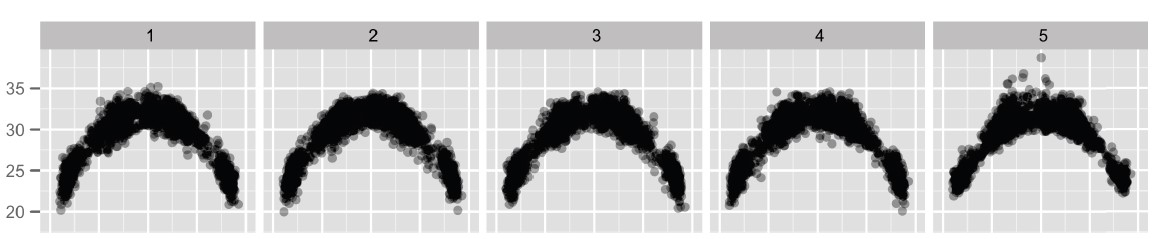
\includegraphics[width=1\linewidth]{ch-visualizer/figures/lineup}
		\caption[A line-up test for $n = 5$. ]{A line-up test for $n = 5$. Consistently identifying the raw data against the synthetic data indicates that the fitted model may not be good enough. Images from Wickham et al. 2010~\cite{wickham2010}}
		\label{fig:visualizer:lineup}
	\end{center}
\end{figure}